\subsubsection{Grain Model}

\paragraph{Cylindrical Grain Model}

A cylindrical grain model was used for rapid exploration and analysis of different sized grains due to a simple analytical solution to how the burn surface area and port area change as the grain burns back. It was assumed that the regression rate is uniform azimuthally. The grain divided into discrete axial sections such that axial differences in regression rate could still be applied.

\begin{align}
    A_{burn} &= \pi (D_{initial} + r_{total})L\\
    A_{port} &= \frac{1}{4}\pi (D_{initial} + r_{total})^2
\end{align}

\paragraph{Level Set Method - Thomas Satterly}

The level set method was used to analyze the burnback characteristics of complex, 3-D grain geometry. Level set models grain burnback as the propagation of a surface normal to its initial surface. As propagating surfaces intersect or diverge, new shapes are created, making analytically models of complex geometry difficult to derive, whereas the level set method inherently predicts and resolves these interactions. The approach used in implementation is known as the Eulerian approach, in which the propagating surface is placed in a fixed burnback grid of points. By calculating the shortest distance between the surface and each point, the a new surface after the desired amount of burnback can be extrapolated using an isocurve throught the grid \cite{tshokotsha_2016}. An example of a purely 2-D burnback of an arbitrary dual-anchor grain is shown in Figure \ref{fig:finocyleBurnback}.

\begin{figure}[H]
    \centering
    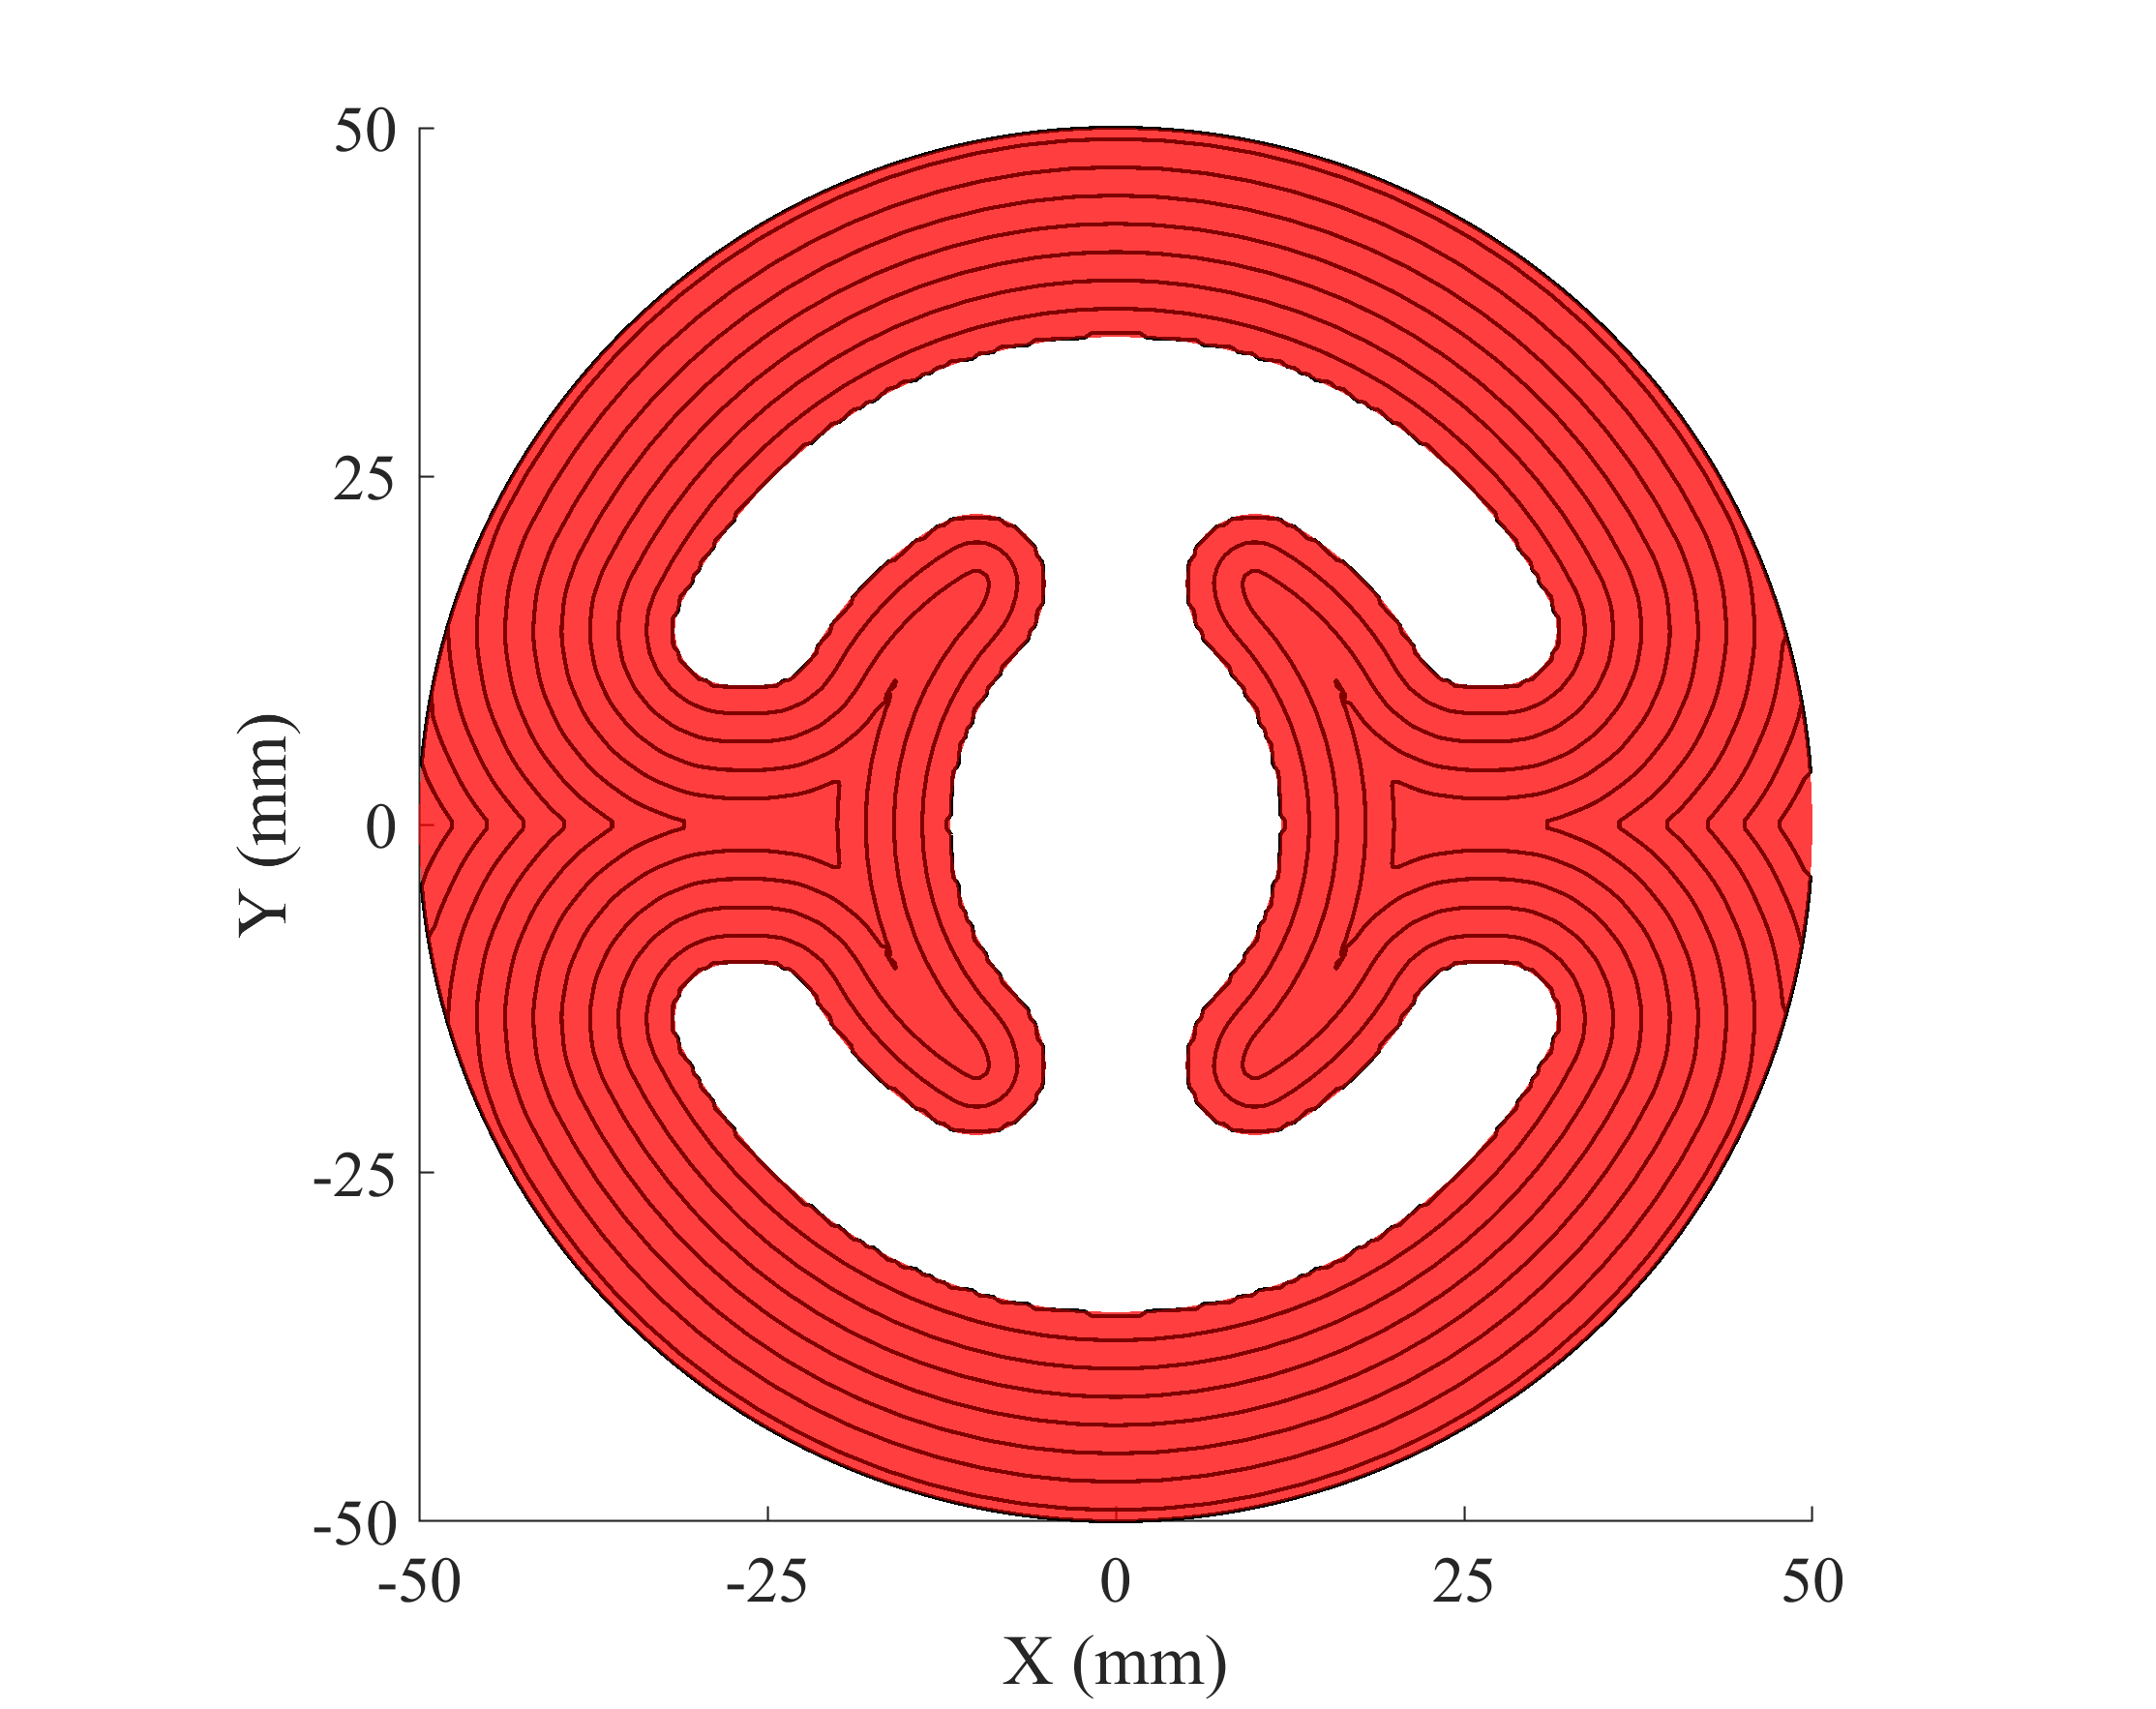
\includegraphics[width=0.7\linewidth]{LevelSet_Figures/anchorGrainBurnback.png}
    \caption{Burnback Levels (2mm steps) of an arbitrary dual-anchor grain}
    \label{fig:finocyleBurnback}
\end{figure}

The model used assumed a uniform azimuthal regression rate and that any axial differences in regression rate could be approximated by axially transforming the burnback grid as appropriate. These assumptions allow for the burnback grid to be pre-computed, saving a significant amount of time during flight simulation. 

\subsubsection{Future Work - Derek Cameron}
\paragraph{Fuel Grain Design}


Going forward into the next steps for the fuel grain design, it would be paramount to pick a better fuel grain shape than just a simple cylinder. A simple cylinder was used in the majority of the calculations that are contained in this report relating to the combustor. This was because a baseline model needed to be used to make sure the code was working. However, there are multiple reasons to pick a different shaped grain.


A cylindrical grain will give a large increase in thrust over time as the burn area is increasing. The thrust increasing is not necessarily an issue, however it will cause our grain to burn out quicker and the thrust increase is just much larger than is needed. Especially if our aerial maneuvers can happen at anytime, not just near the end of the burn where the thrust is the greatest.

For a preferred grain design, work has been done to analyze a finocyl shaped grain. More work needs to be done into designing the exact shape on some of the minor detail of the grain but it shows to have behavior that we deem beneficial. Below is a picture of the cross sectional area of the finocyl grain that has been tested using the level set method discussed previously in this section. The finocyl contains several port areas. These are a great flame holding tactic as the burning area can have further distance from the AeroValve. The ports also allow for a simple igniter method. The igniter can simply be setup to line each port and ignite from there.

\begin{figure}[H]
    \centering
    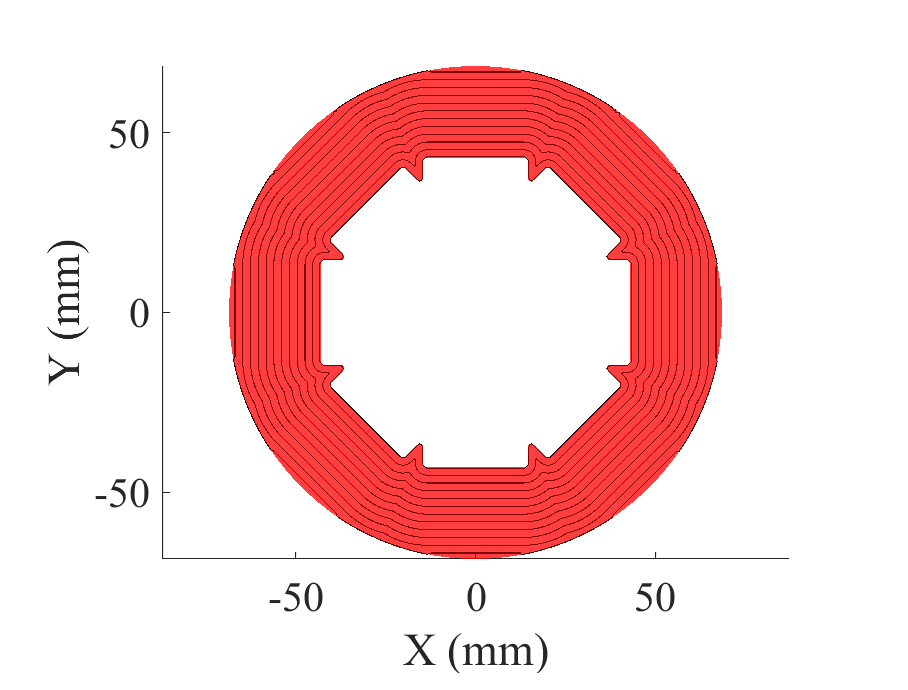
\includegraphics[width=0.7\linewidth]{LevelSet_Figures/FinocylBurnback.eps}
    \caption{Finocyl Grain. Burnback isocontours in 2mm steps}
    \label{fig:finocylgrainshape}
\end{figure}

The burning area vs the over all regression is displayed below for a cylindrical grain. The initial burn area is quite low and then increases to a much larger area. This can lead to having lower thrust in the start of the burn phase. A more extensive design could allow for a longer burn and also better flight control. This cylinder design has the same amount of cross sectional burn area in the beginning of the flight as the finocyl burnback plot shown later in this section. 

\begin{figure}[H]
    \centering
    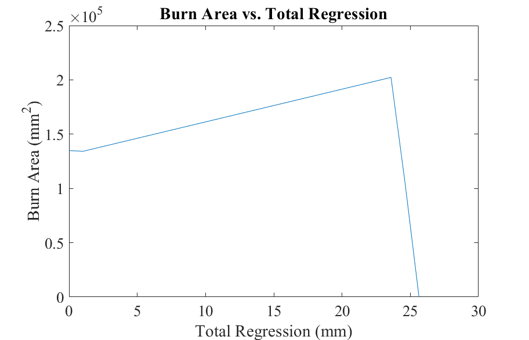
\includegraphics[width=0.7\linewidth]{CombustorDesign/cylindricalgrainburnback.png}
    \caption{Cylindrical grain burnback}
    \label{fig:cylindricalGrainBurnback}
\end{figure}

The next figure is representative of the Finocyl burn area vs. regression. This is a much healthier trending line as the thrust is more constant. There should still be work done to attempt to get a more constant line and remove the dip that occurs in the middle but as can be seen this is a preferred grain shape. The initial burn area of the finocyl shape is much higher than that of the cylindrical one. This allows for higher thrust at the initial burn phase which in turn would allow the SFRJ to make quicker turns and pivots in order to have more control right after the separation of the booster.

\begin{figure}[H]
    \centering
    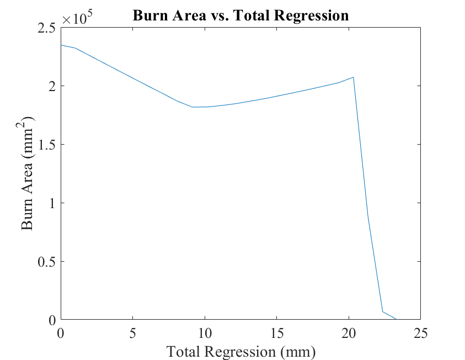
\includegraphics[width=0.7\linewidth]{CombustorDesign/finocylgrainburnback.png}
    \caption{Finocyl grain burnback}
    \label{fig:finocylGrainBurnback}
\end{figure}

The take away for the next step in the fuel grain shape will just be finalizing the grain. If a finocyl shaped grain continues to be the main choice, then the more intricate design choices will need to be made. In the burnback videos of the grains, it is apparent that the current finocyl shape burns a way at the corner of the pockets too quickly. This needs to be solved by either rounding the ports or by changing the port shape. The pointed cusps on the ends of the ports need to be changed. It is unlikely to actually get a pointed cusp in the fuel tank and thus simulating a point such as that can have misleading results. For the final finocyl grain runs, there was a slight arc cut into all of the pointed cusps to give the effect of having them all being curved and not directly pointed. 